
\documentclass{beamer}

\usepackage{hyperref} %for url links
\usepackage{fancyvrb}
\usepackage{graphicx}


%\VignetteIndexEntry{networkDynamic Example}

\usepackage{Sweave}
\begin{document}


\definecolor{Sinput}{rgb}{0.75,0.19,0.19}
\definecolor{Soutput}{rgb}{0,0,0}
\definecolor{Scode}{rgb}{0.75,0.19,0.19}
\DefineVerbatimEnvironment{Sinput}{Verbatim}{formatcom = {\color{Sinput}},fontsize=\footnotesize} 
\DefineVerbatimEnvironment{Soutput}{Verbatim}{formatcom = {\color{Soutput}},fontsize=\footnotesize}
\DefineVerbatimEnvironment{Scode}{Verbatim}{formatcom = {\color{Scode}},fontsize=\small} 
\renewenvironment{Schunk}{}{}
\begin{frame}


\title{A preview of ndtv package for animating dynamic networks}  
\author{Skye Bender-deMoll,\\ Martina Morris}
\maketitle

Statnet workshop
\end{frame}

\begin{frame}[fragile]
\frametitle{Introduction}
Wouldn't it be great if you could actually see the networks you are simulating?

The \verb@ndtv@ package makes movies from \verb@networkDynamic@ objects.

This example runs a very basic \verb@stergm@ simulation.

\end{frame}


\begin{frame}[fragile]
\frametitle{Preparation}


First load in the necessary libraries. 

\begin{Schunk}
\begin{Sinput}
> require(networkDynamic)   # dynamic network extensions
> require(ergm)             # network statistical modeling
> require(sna)              # network descriptive stats
> require(animation)        # animations of R plots
> require(ndtv)             # dynamic network animations
\end{Sinput}
\end{Schunk}

\end{frame}



\begin{frame}[fragile]
\frametitle{Start with a static network}
Load in a very familiar network
\begin{Schunk}
\begin{Sinput}
> data("florentine") # an example network
> plot(flobusiness,displaylabels=T)
\end{Sinput}
\end{Schunk}

\begin{figure}
  \centering
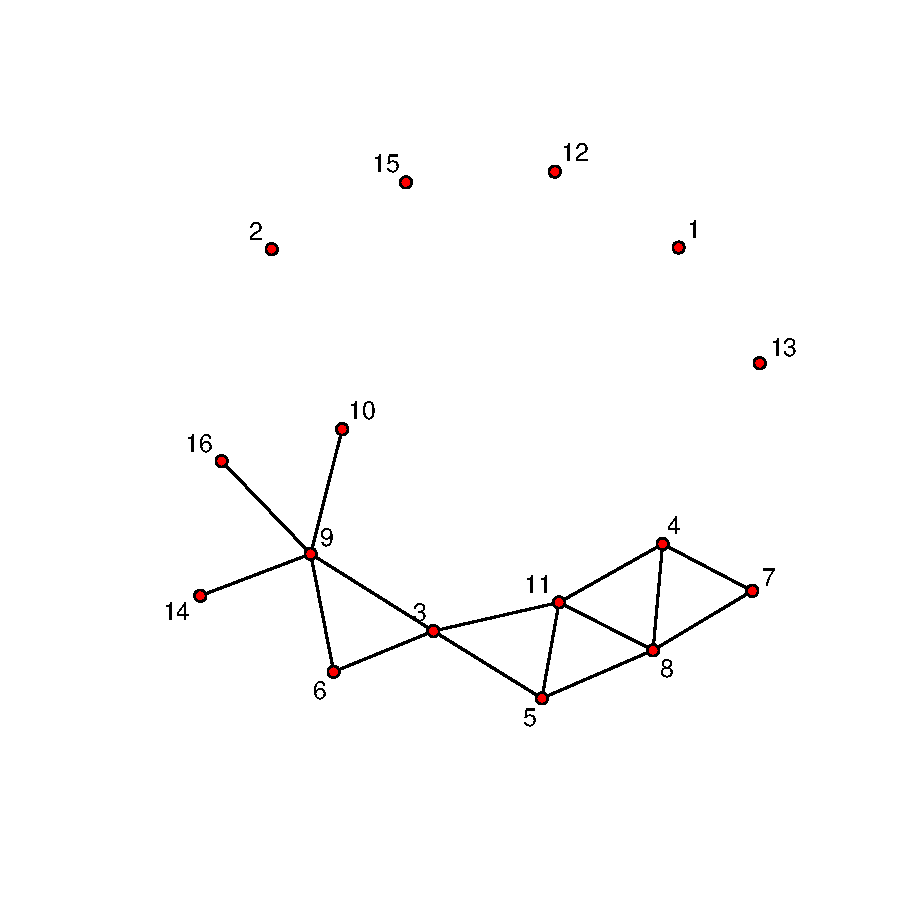
\includegraphics{ndtvDemo-load_net}

\caption{The Florentine Biz network}
\end{figure}

\end{frame}
\begin{frame}[fragile]
\frametitle{Estimate a model}
Define basic \verb@stergm@ model with formation and dissolution parameters.
\begin{Schunk}
\begin{Sinput}
> theta.diss <- log(9)
> stergm.fit.1 <- stergm(flobusiness, # fit stergm
+   formation= ~edges+gwesp(0,fixed=T),
+ 	dissolution = ~offset(edges),
+ 	targets="formation",
+ 	offset.coef.diss = theta.diss,
+ 	estimate = "EGMME"	)
\end{Sinput}
\end{Schunk}
(time passes, lots simulation status output)
\end{frame}




\begin{frame}[fragile]
\frametitle{Simulate from the model}
Simulates 100 discrete time steps from the model and saves them as a \verb@dynamicNetwork@ object.
\begin{Schunk}
\begin{Sinput}
> stergm.sim.1 <- simulate.stergm(stergm.fit.1,
+                     nsim=1, time.slices = 100)
\end{Sinput}
\end{Schunk}
(this is fast!)
\end{frame}

\begin{frame}[fragile]
\frametitle{Render the movie}
We give some parameters to say what time range to render, and ask it to build the animation.

\begin{Schunk}
\begin{Sinput}
> render.par=list(tween.frames=5,show.time=T,
+                 show.stats="~edges+gwesp(0,fixed=T)")
> render.animation(stergm.sim.1,render.par=render.par,
+                  edge.col="darkgray",displaylabels=T,
+                  label.cex=.6,label.col="blue")
\end{Sinput}
\end{Schunk}
(this takes some times, produces output)
\end{frame}
\begin{frame}[fragile]
\frametitle{Action!}
Replay the movie in an R plot window
\begin{Schunk}
\begin{Sinput}
> ani.replay()
\end{Sinput}
\end{Schunk}

Here is a url to the movie:
\url{http://csde.washington.edu/~skyebend/sna_health/stergm.sim.1.mp4}

\end{frame}

\begin{frame}[fragile]
\frametitle{Save the movie}
Use the \verb@animation@ library to save out the movie in \verb@.mp4@ format (using ffmpeg).

\begin{Schunk}
\begin{Sinput}
> saveVideo(ani.replay(),video.name="stergm.sim.1.mp4", 
+                     other.opts="-b 5000k",clean=TRUE)
\end{Sinput}
\end{Schunk}
\end{frame}


\begin{frame}[fragile]
\frametitle{The Details}
There is a bit more going on under the hood.
\begin{itemize}
\item \verb@compute.animation@ extracts sequence of networks, applies layouts, stores coordinates in network
\item \verb@render.animation@ plots using \verb@plot.network@ on stored coords, computes tween frames
\item \verb@animation@ library provides plot caching, and outputs as video in multiple formats.
\end{itemize}
\end{frame}

\begin{frame}[fragile]
\frametitle{The Fine Print}
We chose an easy network to demo
\begin{itemize}
\item Real-world networks harder than simulation output
\item This is an easy network because it is discrete, small, sparse, no node dynamics
\item Saving the videos to disk requires installing some additional non-R software.
\item It currently doesn't scale very well, limited to ~1000 vertices
\end{itemize}
\end{frame}

\begin{frame}[fragile]
\frametitle{Features}
\begin{itemize}
\item Can plugin in multiple layout types
\item Can use some common exteral programs to do layouts, like GraphViz and MDSJ
\item Can aggregate network slices from continuous event data
\item Data and functions easily customized in R
\end{itemize}
\end{frame}

\begin{frame}[fragile]
\frametitle{Concurrency and Reachability movie}
This five minute movie is a dynamic representation of an infection spreading through a transmission network over time.
\begin{itemize}
\item Small network extracted from a large simulation
\item Edge timing tweaked to illustrate infection paths
\item Uses multiple layout types
\end{itemize}
\url{http://csde.washington.edu/statnet/movies/}\\
or\\
\url{http://www.youtube.com/watch?v=r3LYA5kirjA}

\end{frame}


\begin{frame}[fragile]
\frametitle{Layouts: Speedy vs. Stable}
\begin{figure}
  \centering
\includegraphics{ndtvDemo-alg_compare}

\end{figure}
\end{frame}
\begin{frame}[fragile]


\frametitle{The  Teaser}

Coming soon to a repository near you!
\begin{itemize}
\item Dynamic attributes of nodes and edges
\item Edit and adjust positions after calculating
\end{itemize}




\end{frame}

\begin{frame}[fragile]
\frametitle{References}
\scriptsize{
\begin{thebibliography}{}

\bibitem[Bender-deMoll et al.(2008)]{dynamicNetwork}
Bender-deMoll, S., Morris, M. and Moody, J. (2008)
\newblock Prototype Packages for Managing and Animating Longitudinal Network Data: dynamicnetwork and rSoNIA
\newblock \emph{Journal of Statistical Software} 24:7.

\bibitem[Hunter et al.(2008b)]{ergm}
Hunter DR, Handcock MS, Butts CT, Goodreau SM, Morris M (2008b). 
\newblock ergm: A Package to Fit, Simulate and Diagnose Exponential-Family Models for Networks. 
\newblock \emph{Journal of Statistical Software}, 24(3). \url{http://www.jstatsoft.org/v24/i03/}. 

\bibitem[Butts(2008)]{network}
Butts CT (2008). 
\newblock network: A Package for Managing Relational Data in R. 
\newblock \emph{Journal of Statistical Software}, 24(2). \url{http://www.jstatsoft.org/v24/i02/}. 

\bibitem[Bender-deMoll and McFarland(2006)]{sonia}
Skye Bender-deMoll and McFarland, Daniel A. (2006) 
\newblock The Art and Science of Dynamic Network Visualization.
\newblock \emph{Journal of Social Structure. Volume 7, Number 2} \url{http://www.cmu.edu/joss/content/articles/volume7/deMollMcFarland/}

\end{thebibliography}
}
\end{frame}


\end{document}
